\subsection{Data Analysis}
\label{sec:analysis_models}
In this section we describe the data analysis module.
This module analyzes the trajectories given by the trajectory extraction module.
%This module consists of two components: common movement discovery and abnormal pattern detection.
The following sub-sections provide the details of this module.

\subsubsection{Common Movement Discovery}
\label{sec:common_movement_discovery}
Discovering common movements is a critical process for exploration and analysis of a large volume of trajectory data.
%where the entities that need to be analyzed are trajectories.
Clustering is a popular approach in looking for common patterns in the trajectory data.
%by organizing trajectories into groups whose members are similar in some way.
%A number of clustering algorithms have been proposed by researchers.
Representative clustering algorithms for trajectory include DBSCAN~\cite{Ester:1996:Density} and OPTICS~\cite{Ankerst:1999:Optics}.
Andrienko et al.~\cite{Andrienko:2013:Visual} propose a wide range of clustering-based analytics models and combine those with visualization techniques.
Their clustering models, however, group similar trajectories as a whole and extract common whole trips.
In this work, we utilize a modified partition-based clustering model, TRACLUS~\cite{Lee:2007:Trajectory}, in order to find common sub-trajectories.
For each given trajectory, this model first partitions a trajectory into a set of line segments, and then groups the line segments into clusters of similar line segments.
Clustering the line segments (as opposed to whole trajectories) eables the extraction of similar portion of trajectories.
%Clustering the line segments is very useful, because we can extract common behaviors, even though there is no cluster if the basic unit of clustering is the whole trajectory.
For example, Figure~\ref{fig:common_sub_trajectory} shows that the three trajectories (green, black, red) have different origins and destinations, but there is a common path in all three trajectories (blue).
%This is valuable information.
%We need to discover the common behavior. This is valuable information.
%
%For trajectory partitioning, the existing model utilizes MDL~\cite{Grunwald:2005:Advances} to find characteristic points that change the direction rapidly from all points of each trajectory.
%In this work, however, the points resulting from the way are too spares to partition the trajectories into appropriate line segments.
%Therefore, we use the series of the waypoints resulting from the route direction calculation service described in Section~\ref{sec:trajectory_extraction} in order to gain adequately fine-grained characteristic points.
%, for example, the black dots of each trajectory in Figure~\ref{fig:common_sub_trajectory}.

\begin{figure}[tb]
	\centering
	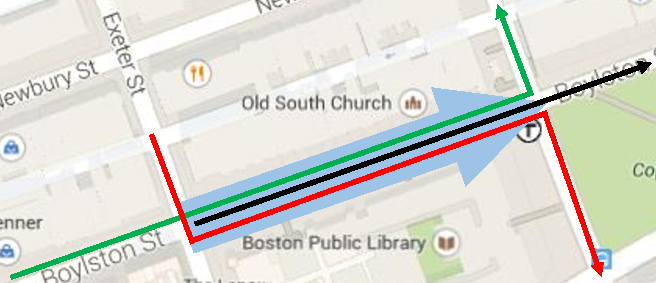
\includegraphics[width=0.8\linewidth]{common_sub_trajectory_v2}
	\caption{Discovering a common sub-trajectory.}
	\label{fig:common_sub_trajectory}
	%\vspace{-0.4cm}
\end{figure}

Clustering the line segments requires a distance function measuring the distance between line segments.
We use the distance function based on a modified line segment Hausdorff distance~\cite{Chen:2003:Noisy}, which is comprised of three components: the perpendicular distance ($d_\bot$), the parallel distance ($d_\parallel$), and the angle distance ($d_\theta$).
Let $s_i$ and $e_i$ be the starting and ending points of line $L_i$, and $s_j$ and $e_j$ for line $L_j$.
Without loss of generality, the longer line segment is assigned to $L_i$, and the shorter one to $L_j$.
These are illustrated in Figure~\ref{fig:distancefunction}.

For our distance function, we use $d_\bot$ and $d_\parallel$ as defined by ~\cite{Chen:2003:Noisy}, but redefine $d_\theta$ as the existing model does not consider the directions of the two line segments for the angle distance measure.
In this work direction is an important factor in clustering and abnormal movement detection.
To consider the direction, we utilize the cosine-similarity that measures the cosine of the angle between line segments, and is used as a bounded similarity function within $[0,1]$. 
$d_\theta(L_i, L_j)$ is defined as:
%This is different from ~\cite{Lee:2007:Trajectory}.
%The angle distance:
\begin{equation}
\begin{aligned}
d_\theta(L_i, L_j) = \parallel L_j \parallel \times \frac{\cos^{-1} (\mathit{cosine\mbox{-}similarity}(L_i, L_j))} {\pi}
\end{aligned}
\end{equation}
where $\parallel L_j \parallel$ denote length of $L_j$, and $\theta$ $(0^{\circ} \le \theta \le 180^{\circ})$ denote the smaller intersecting angle between $L_i$ and $L_j$, and $\mathit{cosine\mbox{-}similarity}(L_i, L_j)$ is defined as:
\begin{equation}
\mathit{cosine\mbox{-}similarity}(L_i, L_j) = \cos (\theta) = 
\frac{\overrightarrow{s_i e_i} \cdot \overrightarrow{s_j e_j} } {\parallel \overrightarrow{s_i e_i} \parallel \parallel \overrightarrow{s_j e_j} \parallel}	
\end{equation}
$\parallel L_j \parallel$ denote length of $L_j$, and $\theta$ $(0^{\circ} \le \theta \le 180^{\circ})$ denote the smaller intersecting angle between $L_i$ and $L_j$.


%The perpendicular distance:
%\begin{equation}
%d_\bot(L_i, L_j) = \frac{l_{\bot1}^2 + l_{\bot2}^2}{l_{\bot1} + l_{\bot2}}
%\end{equation}
%where $p_s$ and $p_e$ are the projection points of the points $s_j$ and $e_j$ onto $L_i$, respectively. 
%$l_{\bot1}$ is the Euclidean distance between $s_j$ and $p_s$; $l_{\bot2}$ is that between $e_j$ and $p_e$.
%
%The parallel distance:
%\begin{equation}
%d_\parallel(L_i, L_j) = MIN(l_{\parallel1}, l_{\parallel2})
%\end{equation}
%where $l_{\parallel1}$ is the Euclidean distances of $p_s$ to $s_i$ and $l_{\parallel2}$ is that of $p_e$ to $e_i$.

%where
%\begin{align*}
%\mathit{cosine\mbox{-}similarity}(L_i, L_j) = \cos (\theta) = 
%\frac{\overrightarrow{s_i e_i} \cdot \overrightarrow{s_j e_j} } {\parallel \overrightarrow{s_i e_i} \parallel \parallel \overrightarrow{s_j e_j} \parallel}	
%\end{align*}

%\begin{equation}
%\begin{aligned}
%d_\theta(L_i, L_j) = \parallel L_j \parallel \times \frac{\cos^{-1} (\mathit{cosine\mbox{-}similarity}(L_i, L_j))} {\pi}, \enspace \mathrm{where} \\
%\mathit{cosine\mbox{-}similarity}(L_i, L_j) = \cos (\theta) = 
%\frac{\overrightarrow{s_i e_i} \cdot \overrightarrow{s_j e_j} } {\parallel \overrightarrow{s_i e_i} \parallel \parallel \overrightarrow{s_j e_j} \parallel}	
%\end{aligned}
%\end{equation}


The distance function is finally defined as the sum of three components:
\begin{equation}
\label{eq:distancefunction}
\begin{aligned}
dist(L_i, L_j) = w_\bot \cdot d_\bot(L_i, L_j) + w_\parallel \cdot d_\parallel(L_i, L_j) + w_\theta \cdot d_\theta(L_i, L_j)
\end{aligned}
\end{equation}
where $w_\bot$, $w_\parallel$, and $w_\theta$ are weight values, which are determined depending on applications.

\begin{figure}[tb]
	\centering
	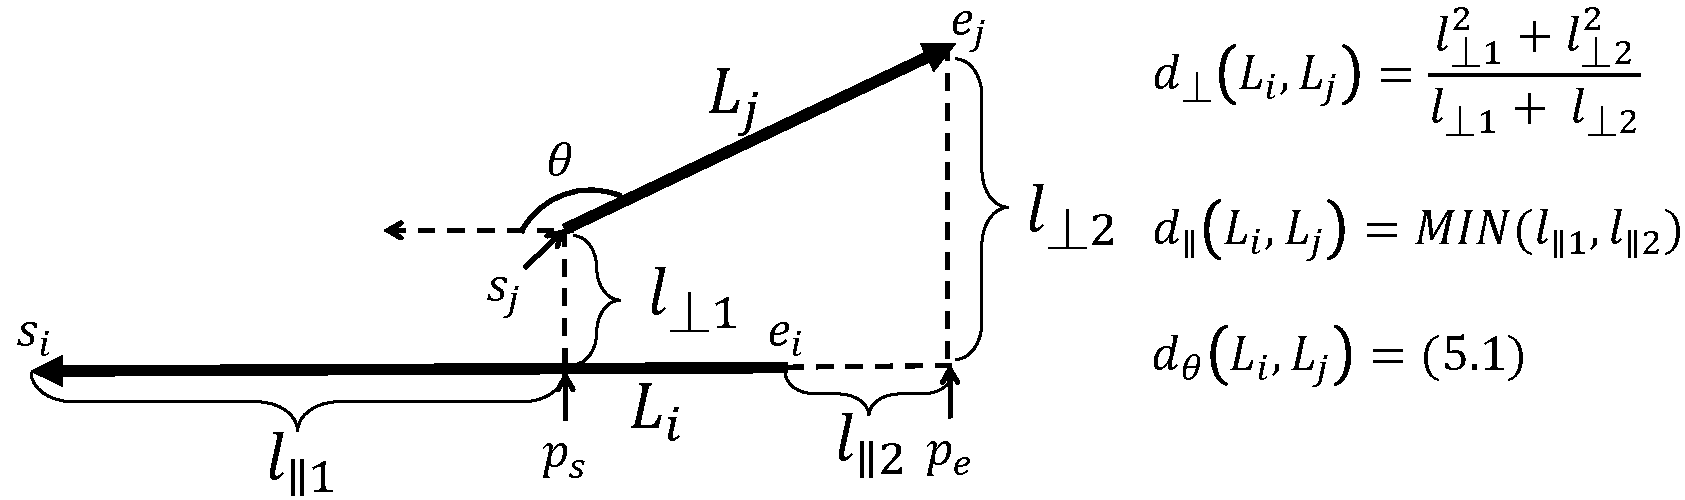
\includegraphics[width=1.0\linewidth]{distancefunction_v3}
	\caption{Similarity measurement for two line segments.}
	\label{fig:distancefunction}
	%\vspace{-0.4cm}
\end{figure}

The partition-based clustering model utilized in this work is based on the algorithm DBSCAN~\cite{Ester:1996:Density}.
Given a set of line segments, the algorithm groups the line segments into a set of clusters according to the distance function Equation (\ref{eq:distancefunction}).
DBSCAN requires two parameters: $\epsilon$ (as neighborhood distance) and $MinLns$ (as minimum cluster size).
The clustering model estimates the optimal parameter values based on input data.
An initial result generated by the estimated parameters is given to users.
However, the automatically estimated parameter values do not always provide optimal results.
Especially, $MinLns$ relies on user's domain knowledge and application requirements.
So, our system allows the users to manually adjust the estimated values.
The system then generates a representative trajectory for each cluster, which epitomizes the line segments (sub-trajectories) belonging to the corresponding cluster. More detailed information about these procedures can be found in ~\cite{Lee:2007:Trajectory}.


\subsubsection{Abnormal Movement Detection}
\label{sec:abnormal_movement_detection}
Existing anomaly detection models~\cite{Liao:2010:Anomaly,Lee:2008:Trajectory} for trajectory data have mainly focused on identifying outliers from a target dataset.
The models are usually based on non-supervised learning\textemdash they generally do not have factors for the outliers, and assume that the outliers make for a small sub-set from the entire dataset.
These models first look for major flow patterns and then determine whether each trajectory belongs to the majority according to specific criteria.
However, during abnormal situations, such as natural disasters and crisis events, even the major behaviors can be unusual compared to normal situations.

In this work, we propose a classification model based on historical data for abnormal movement detection using human expert interaction.
We allows the users to utilize their domain knowledge of the geographical and temporal characteristics of the location where an abnormal event of interest occurs.
The users select a target time window for the abnormal situation and also chooses another time window representing a normal/regular situation for the location.
%We expect the users of our system have knowledge about the location that need to be analyzed, such as regular or special events and temporal characteristics the location.
%We combine such human expert knowledge with our analytics model to detect abnormal movement.
%Our system requires not only a target time window to be analyzed, but also a past time window representing a normal/regular situation of the location from the users for comparison between the two situations.
We extract two sets of trajectories for the two different time frames and cluster each set of trajectories into two sets of trajectory clusters.
Next, we generate two different sets of representative trajectories: target $T$ and comparable $C$.
A representative trajectory $RT_{ti} \in T$ is classified as an outlier if there is a close representative trajectory $RT_{ci} \in C$.
More specifically, we identify outlying line segments $L_{ti} \in RT_{ti}$~\cite{Lee:2008:Trajectory}, which are determined by the distance from neighboring $RT_{ci}$.
We define a representative trajectory $RT_{ci}$ is close to a line segment $L_{ti}$ if $\sum_{L_{ci} \in CRT_{c}} len(L_{ci}) \leq len(L_{ti}) $ where $CRT_{c}$ is the set of $RT_{ci}$'s line segments within the distance $D$ from $L_{ti}$, $\left\{L_{ci} \enspace| \enspace dist(L_{ci}, L_{ti}) \leq D\right\}$. 
A larger value of $D$ detects a smaller number of outliers, and a smaller value of $D$ a larger number of outliers.
Then, intuitively a representative trajectory $RT_{ti}$ is outlying, if the percentage of the total length of outlying line segments is more than $P$. The default value of $P$ is set to 30.
Finally, the outlying representative trajectories are visualized.
Our system allows the users to adjust the two parameter values, $D$ and $P$ in order to refine their results.



